\documentclass[xcolor=dvipsnames]{beamer}

\DeclareMathAlphabet{\mathpzc}{OT1}{pzc}{m}{it}

\usepackage{verbatim, mathrsfs, dsfont, multirow, ulem, pifont, pgf, tikz, verbatim, graphicx, bbding, multicol, xcolor, fancybox, mdframed, amsmath, alltt, booktabs,tikz,hyperref}

\usetikzlibrary{positioning,calc}

\setbeamertemplate{theorems}[numbered]
\setbeamertemplate{footline}{\color{Blue} \hspace{.1in}\insertframenumber/\inserttotalframenumber \vspace{.1in}}

\newcommand*{\vctr}[1]{\begingroup
\setbox0=\hbox{#1}\parbox{\wd0}{\box0}\endgroup}

\makeatletter
\long\def\beamer@@frametitle[#1]#2{
  \beamer@ifempty{#2}{}{
    \gdef\insertframetitle{\centering{#2\ifnum\beamer@autobreakcount>0\relax{}\space\usebeamertemplate*{frametitle continuation}\fi}}
  \gdef\beamer@frametitle{#2}
  \gdef\beamer@shortframetitle{#1}
}
}
\makeatother

\mode<presentation>
{
  \usetheme{JuanLesPins}
  \usecolortheme{dolphin}
  %%%\usefonttheme{structuresmallcapsserif}
  %%%\usefonttheme[onlylarge]{structurebold}
  \usefonttheme{serif}
  \setbeamercovered{invisible}
}


\usepackage[english]{babel}
\usepackage[latin1]{inputenc}
\usepackage{times}
\usepackage[T1]{fontenc}
% Or whatever. Note that the encoding and the font should match. If T1
% does not look nice, try deleting the line with the fontenc.

\tikzset{onslide/.code args={<#1>#2}{%
  \only<#1>{\pgfkeysalso{#2}} % \pgfkeysalso doesn't change the path
}}

\newcommand<>{\superimpose}[2][]{%
  \tikz[overlay, remember picture]{%
    \filldraw#3[blue!30,opacity=0.5](current page.north west) rectangle (current page.south east);
    \node#3[at=(current page),#1]{#2};
  }%
}


\title{Welcome to class!}

\author{{ with Prof. J. D'Ambroise} }


% If you wish to uncover everything in a step-wise fashion, uncomment
% the following command:
%\beamerdefaultoverlayspecification{<+->}
\date{}

%%%\subject{Talks}
% This is only inserted into the PDF information catalog. Can be left
% out.



% If you have a file called "university-logo-filename.xxx", where xxx
% is a graphic format that can be processed by latex or pdflatex,
% resp., then you can add a logo as follows:

% \pgfdeclareimage[height=0.5cm]{university-logo}{university-logo-filename}
% \logo{\pgfuseimage{university-logo}}


% \begin{comment}
% \begin{frame}{Make Titles Informative.}
%   You can create overlays\dots
%   \begin{itemize}
%   \item using the \texttt{pause} command:
%     \begin{itemize}
%     \item
%       First item.
%       \pause
%     \item
%       Second item.
%     \end{itemize}
%   \item
%     using overlay specifications:
%     \begin{itemize}
%     \item<1->
%       First item.
%     \item<2->
%       Second item.
%     \end{itemize}
%   \item
%     using the general \texttt{uncover} command:
%     \begin{itemize}
%       \uncover<5->{\item
%         First item.}
%       \uncover<6->{\item
%         Second item.}
%     \end{itemize}
%   \end{itemize}
% \end{frame}
% \subsection{Second Subsection}
% \begin{frame}{Make Titles Informative.}
% \end{frame}
% \begin{frame}{Make Titles Informative.}
% \end{frame}
% \section*{Summary}
% \begin{frame}{Summary}
%   % Keep the summary *very short*.
%   \begin{itemize}
%   \item
%     The \alert{first main message} of your talk in one or two lines.
%   \item
%     The \alert{second main message} of your talk in one or two lines.
%   \item
%     Perhaps a \alert{third message}, but not more than that.
%   \end{itemize}
%   % The following outlook is optional.
%   \vskip0pt plus.5fill
%   \begin{itemize}
%   \item
%     Outlook
%     \begin{itemize}
%     \item
%       Something you haven't solved.
%     \item
%       Something else you haven't solved.
%     \end{itemize}
%   \end{itemize}
% \end{frame}
% \end{comment}

% Delete this, if you do not want the table of contents to pop up at
% the beginning of each subsection:
%%%\AtBeginSubsection[]
%%%{
  %%%\begin{frame}<beamer>{Outline}
    %%%\tableofcontents[currentsection,currentsubsection]
  %%%\end{frame}
%%%}

% If you wish to uncover everything in a step-wise fashion, uncomment
% the following command:

%\beamerdefaultoverlayspecification{<+->}


%AN XY PIC EXAMPLE, IN CASE WANT TO DRAW ARROWS


\begin{document}

% For every picture that defines or uses external nodes, you'll have to
% apply the 'remember picture' style. To avoid some typing, we'll apply
% the style to all pictures.

% By default all math in TikZ nodes are set in inline mode. Change this to
% displaystyle so that we don't get small fractions.
\everymath{\displaystyle}

\section{High Expectations}


\begin{frame}{\bf Failing Mentality\\ (for lack of a better word)}

\begin{itemize}
\item go to class
\item do assignments
\item take exams
\end{itemize}

\end{frame}


\begin{frame}{ \bf Mentality for Success:\\ learn to engage \& think in new ways}

\begin{itemize}
\item {\color{blue} prepare in advance}
\item go to class
\item {\color{blue} discuss with your peers \& communicate with prof.}
\item do assignments
\item {\color{blue} think, ponder, ask questions, review, revise}
\item take exams
\item {\color{blue}  be realistic \& evaluate your progress honestly} 
\end{itemize}

\begin{center}
{\color{purple}
{\it Be prepared to work outside your comfort zone!}
}
\end{center}

\end{frame}


\begin{frame}{\bf You will need to master... }

BIG IDEAS (big scale)
\begin{itemize}
\item how math relates to real life
\item how to read and interpret math
\item understanding different presentations of the same information
\end{itemize} 

\vspace{.2in}
STEPS OF PROBLEMS (small scale)
\begin{itemize}
\item algebra 
\item trig 
\item graphing functions
\item prerequisite material
\item new material
\end{itemize}

\end{frame}


\begin{frame}{\bf Communication is key}


Office hours
\begin{itemize}
\item basic algebra questions
\item basic trig questions
\item basics about how to graph a function 
\item questions about prerequisite material you forgot
\item questions about what we are currently covering
\item questions about your major / your life goals, etc.
\item and more!
\end{itemize}

\end{frame}


\section{Harmful Math Stereotypes}


\begin{frame}{\bf Harmful Math Stereotypes}

\begin{itemize}
\item "I am not a math person."
\pause
\begin{quote}\begin{center}
{\color{blue}
"Math people" are not born, they are created.\\
Math is a SKILL not a talent. \\ 
\pause
\ \\
It's a vicious cycle:\\ if you believe you cannot do math,\\ then you won't work hard enough \& you won't do well,\\ then your false belief that you can't do it will be verified!  \\
\pause
\ \\
BREAK THE CYCLE\\ by working hard\\ and learning to communicate \& ask for help.
}
\end{center}\end{quote}
\end{itemize}

\end{frame}


\begin{frame}{\bf Harmful Math Stereotypes}

\begin{itemize}
\item "I just CANNOT read a math textbook."
\pause
\begin{quote}\begin{center}
{\color{blue}
Don't handicap yourself by adopting \\ false beliefs about your abilities.\\
Work hard and LEARN HOW to read a math textbook.\\
\ \\
Tips: Skipping around is recommended for math!  \\
(math textbook $\neq$ novel)\\
 Be persistent, ask questions, take notes. \\ Actively engage, don't be passive.
}
\end{center}\end{quote}
\pause
\item Math is an Inborn Talent 
\pause 
\begin{quote}\begin{center}
{\color{blue}
False. \\ 
Math is an acquired skill that takes \\
hard work and dedication.
}
\end{center}\end{quote}
\end{itemize}

\end{frame}


\begin{frame}{\bf Harmful Math Stereotypes}

\begin{itemize}
\item The Lone Genius 
\pause 
\begin{quote}\begin{center}
{\color{blue}
Everyone is different, but the majority  \\
research Mathematicians THRIVE\\
 on communication and teamwork!\\
 \pause
 \ \\
 Don't handicap yourself by\\ shutting out peers, the prof., tutors, etc..\\
 \ \\ 
 Communication is essential to learning math!

}
\end{center}\end{quote}
\end{itemize}

\end{frame}


\begin{frame}{\bf Harmful Math Stereotypes}

\begin{itemize}
\item Smart people don't make mistakes
\pause 
\begin{quote}\begin{center}
{\color{blue}
 FALSE!\\
Students who do well take the time to ask about: algebra, trig, other basics, prerequisite material, etc.
}
\end{center}\end{quote}
\pause
\item The Prof. will look down on me if I ask a question about basics 
\pause 
\begin{quote}\begin{center}
{\color{blue}
There are NO dumb questions in this class!\\
Students asking questions are showing initiative!\\
The Prof. loves working one-on-one for the best result!
}
\end{center}\end{quote}
\end{itemize}

\end{frame}






\begin{frame}{\bf Mentality for Success}

\begin{center}
{\LARGE{\color{blue}
Too proud to get help?\\
Too scared to get help?\\
Too busy to get help?}}\\
\pause
\ \\
{\LARGE {\color{red}
You're at risk for failure. }}
\end{center}

\end{frame}


\section{ Advice From Students}


\begin{frame}{\bf Advice From Students}

"I wish I hadn't taken this class while ...\\
\pause
\begin{itemize}
\item ... taking organic chemistry."
\pause
\item ... running 3 businesses."
\pause
\item ... working full time."
\pause
\item ... struggling with a drug problem."
\pause
\item ... my schedule was so tight there was no time for crucial office hours, appointments, or tutoring that I really needed."
\pause
\end{itemize}

\begin{quote}\begin{center}
{\color{blue}
This class is a commitment.\\ Plan wisely.}
\end{center}\end{quote}

\end{frame}


\begin{frame}{\bf Advice From Students}

"I had no idea ...\\
\pause
\begin{itemize}
\item ... finishing HW early helps with understanding the material."
\pause
\begin{quote}\begin{center}
{\color{blue}
WHY?\\ Higher math is conceptual.\\ Your brain needs time to settle and absorb it.
}
\end{center}\end{quote}
\pause
\item ... making study sheets helps with understanding the concepts."
\pause
\begin{quote}\begin{center}
{\color{blue}
WHY?\\ There is A LOT of information in this class.\\ Quick summaries help to reduce the cognitive load.
}
\end{center}\end{quote}
\end{itemize}

\end{frame}


\begin{frame}{\bf Advice From Students}

"I had no idea ...\\
\pause
\begin{itemize}
\item ... working in peer groups is actually helpful\\  \ \ \  \ \ \ \ (I thought it would be annoying and/or stressful)."
\pause
\begin{quote}\begin{center}
{\color{blue}
WHY?\\  Other students can help when you don't understand.\\   Helping others will increase your math confidence!\\ You'll see other students have the same questions.
}
\end{center}\end{quote}
\pause
\item ... a quick meeting with the Prof. actually cleared up things I had been confused about for months."
\pause
\begin{quote}\begin{center}
{\color{blue}
WHY?\\  After over a decade of teaching, the Prof. has seen many many students struggle and succeed past the same issues you are dealing with !  
}
\end{center}\end{quote}
\end{itemize}

\end{frame}


\section{Five Stages of Learning}


\begin{frame}{\bf Five Stages of Learning}

\begin{enumerate}
\item {\bf Novice:} technically knows the rules but has little or no situational understanding and cannot adapt quickly
\pause
\item {\bf Competent:}  understands different situations, exceptions, or deviations from the rules
\pause
\item {\bf Proficient:}  focuses is on long term goals (relating math to your major) rather than difficulties of individual math problems
\pause
\item {\bf Expert:}  rules are instinctual \& automatic, student has practiced so much they not surprised by exam questions
\pause
\item {\bf Mastery:}  (rare) mental energy no longer needed to produce nearly perfect results
\end{enumerate}

\end{frame}

\begin{frame}{\bf Five Stages of Learning:  {\color{blue} GOALS for exams }}

\begin{enumerate}
\item {\color{red} (fail)} {\bf Novice:} technically knows the rules but has little or no situational understanding and cannot adapt quickly
\pause
\item {\color{red} (fail)} {\bf Competent:}  understands different situations, exceptions, or deviations from the rules
\pause
\item {\color{blue} (possible pass)} {\bf Proficient:}  focuses is on long term goals (relating math to your major) rather than difficulties of individual math problems
\pause
\item {\color{blue} (decent outcome: A or B)} {\bf Expert:}  rules are instinctual \& automatic, student has practiced so much they not surprised by exam questions
\pause
\item {\color{blue} (decent outcome: A or B)} {\bf Mastery:}  (rare) mental energy no longer needed to produce nearly perfect results
\end{enumerate}

\end{frame}


\section{Get Motivated}


\begin{frame}{\bf Memes}

\begin{center}

\includegraphics[width=2in]{comfortzone.jpg} \ \ \

\includegraphics[width=2in]{noelevator.jpg}
\end{center}

\end{frame}


\begin{frame}{\bf Everyday}

\begin{center}

\includegraphics[width=3.5in]{tryharder.jpg}
\end{center}

\end{frame}


\section{Extra Info}


\begin{frame}{}

\begin{center}
{\color{gray} The next few pages are designed for courses with online HW.}\\

\includegraphics[width=2in]{asciibunny.png}\\
{\color{gray} The next few pages are designed for courses with online HW.}
\end{center}

\end{frame}


\begin{frame}{}

\begin{center}
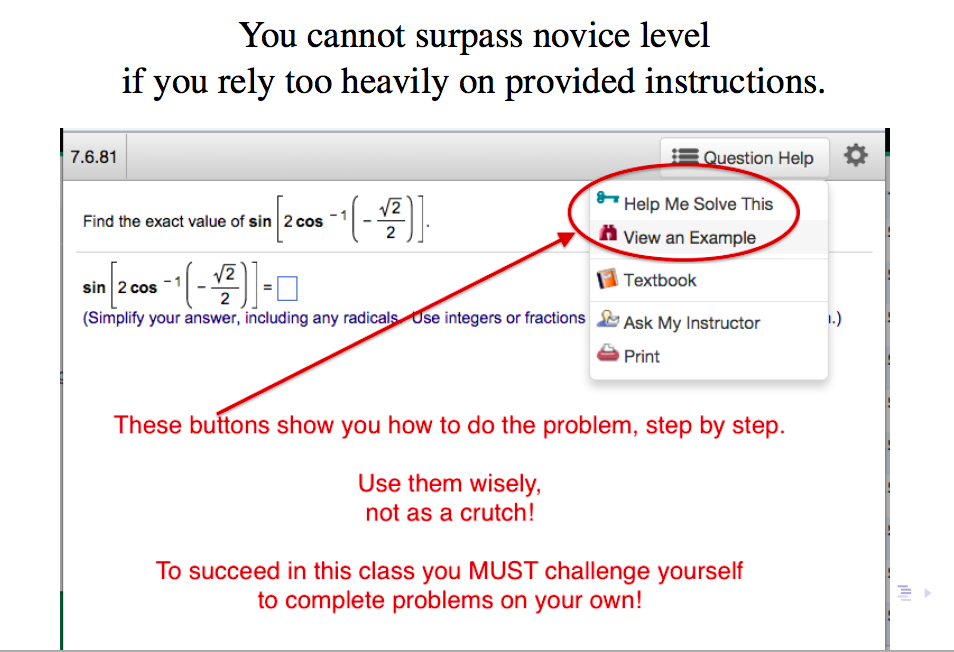
\includegraphics[width=4in]{CalcNovice.png}
\end{center}

\end{frame}


\begin{frame}{}

\begin{center}
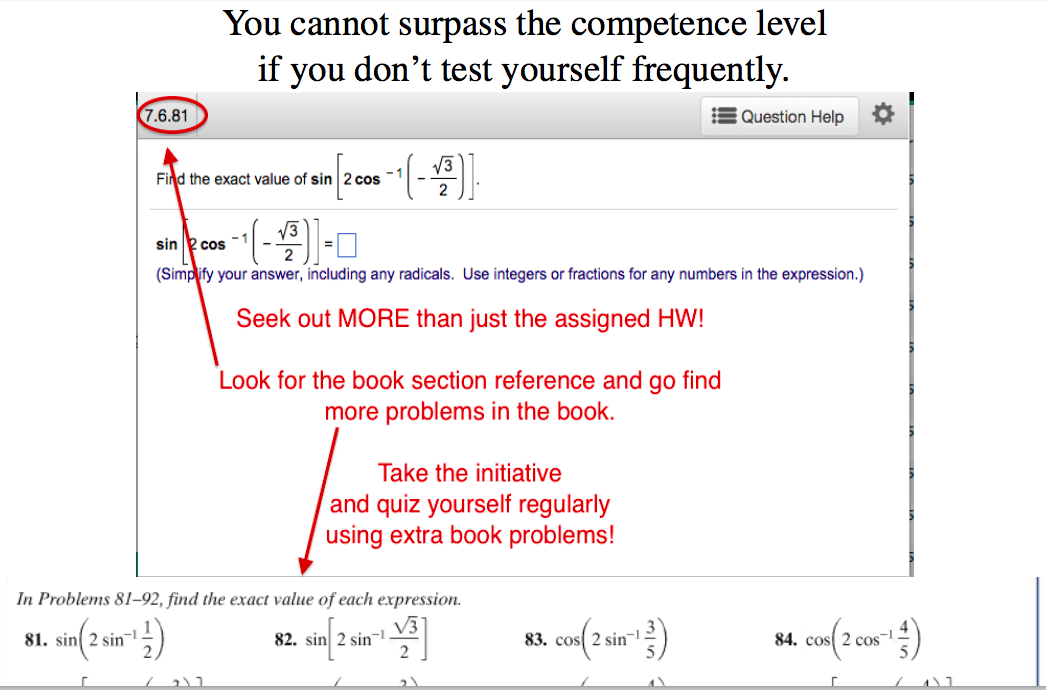
\includegraphics[width=4in]{CalcCompetent.png}
\end{center}

\end{frame}









\end{document}
